\section{Atomic Structure}
Electrons, and all matter, behave like waves, which can undergo constructive and destructive
interference.

\begin{tabularx}{\linewidth}{|l|X|l|} \hline
    \multicolumn{3}{|c|}{$\lambda = \frac{h}{mv}$} \\ \hline
    & \textbf{value} & \textbf{unit} \\ \hline
    $\lambda$ & De Broglie wavelength & m \\ \hdashline
    $h$ & Planck's constant $= 6.626 \times 10^{-34}$& J/s \\
    $m$ & particle mass & \si{\kilo\gram} \\
    $v$ & particle velocity & \si{\metre\per\sec}\\ \hline
\end{tabularx}

By \textbf{Heisenberg's uncertainty principle}, it is impossible to know the precise position
of electrons in an atom.

\subsection{Quantum Mechanical Model}
A \textbf{wave equation} describes the behavior of a specific electron in an atom.

The solution to the wave equation is called a \textbf{wave function} ($\psi$), 
or an \textbf{orbital} --- the space boundary where there is a 95\% chance of finding the electron.

$|\psi|^2$ is proportional to the \emph{probability density} of an electron being found in 3D space.

The position of an electron could be described using \textit{Cartesian coordinates}, using the wave
equation $\psi(x, y, z)$.

Alternatively, using \textit{spherical coordinates}, $\psi(r, \theta, \phi)$:

\begin{tabularx}{\linewidth}{|l|X|l|} \hline
    \multicolumn{3}{|c|}{$\psi(r, \theta, \phi) = \mathbf{R}(r) \times \mathbf{Y}(\theta, \phi)$} \\ \hline
    & \textbf{value} & \textbf{unit} \\ \hline
    $\mathbf{R}(r)$ & \textbf{radial wave function} & -- \\
    $r$ & distance of the electron from the nucleus & -- \\ \hdashline
    $\mathbf{Y}(\theta, \phi)$ & \textbf{angular wave function} & -- \\
    $\theta$ & vertical angle perpendicular to the $x$-$y$ plane & -- \\
    $\phi$ & angle on the $x$-$y$ plane & -- \\ \hline
\end{tabularx}

\textbf{Radial nodes} are 3D \textit{spherical} regions where where no electrons are found.
The \textit{radial} component of the wave function passes through 0.

\textbf{Angular nodes} are 2D \textit{planar} or 3D \textit{conical} regions where where no electrons are found.
The \textit{angular} component of the wave function passes through 0.

In orbital diagrams, the regions corresponding to positive values of the wave function are shaded,
while the regions corresponding to negative values are not.

\subsubsection{Radial Distribution Function (RDF)}
\begin{tabularx}{\linewidth}{|l|X|l|} \hline
    \multicolumn{3}{|c|}{$RDF: 4 \pi r^2 \cdot \mathbf{R}(r)^2$ } \\ \hline
    & \textbf{value} & \textbf{unit} \\ \hline
    $4 \pi r^2$ & surface area of a sphere & -- \\
    $\mathbf{R}(r)$ & radial wave function & -- \\ \hline
\end{tabularx}

\vspace*{1em}
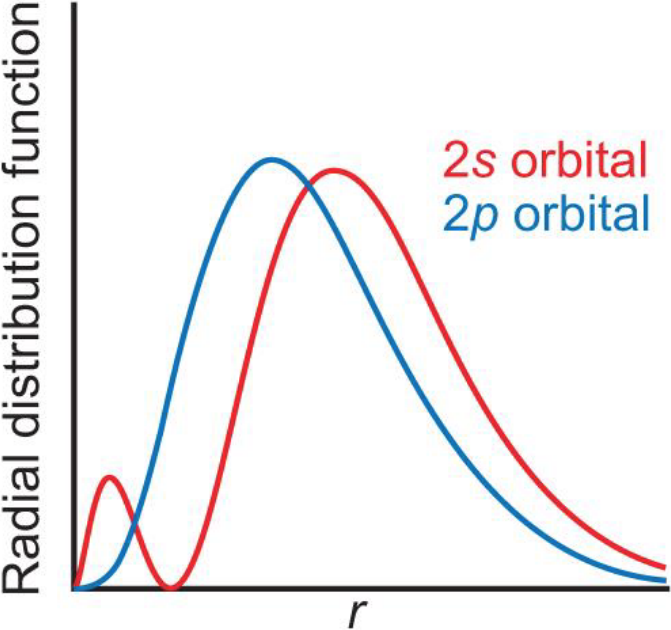
\includegraphics[width=\linewidth/2]{rdf}

The maximum value of the RDF (i.e. the peak) is the most probable distance of the electron
from the nucleus.

Even though the larger peak of the $2p$ orbital is closer than that of the $2s$ orbital,
the $2s$ orbital has a higher energy level than the $2p$ orbital due to the \textbf{penetration}
from the smaller peak.

Therefore, within shells of the same quantum number, orbital energy increases as follows:
 $s < p < d < f$.

 Radial nodes can be counted from the $x$-intercepts, so from the diagram above,
 the $2s$ orbital has 1 radial node, while the $2p$ orbital has none.

 \subsubsection{Quantum Numbers}
 \begin{tblr}{|l|X|X|} \hline
    \SetCell[c=3]{c} $nl_{m_l}$, e.g. $2p_z$ \\ \hline
    & \textbf{value} & \textbf{range} \\ \hline
    $n$ & principal QN & 1, 2, 3, \dots \\
    $l$ & magnetic QN & 0, 1, \dots, $n-1$ \\
    $m_l$ & {orbital angular \\ momentum QN} & $-l, \dots, 0, \dots, +l$ \\ \hline
\end{tblr}

The principal QN relates to the \textit{size} and \textit{energy} of the orbital --- higher principal QNs
have larger orbitals with higher energy levels.

The magnetic QN relates to the \textit{shape} of the orbital.

The orbital angular momentum QN relates to the \textit{orientation} of the orbital.

\begin{tabularx}{\linewidth}{|Y|c|} \hline
    number of angular nodes & $l$ \\ \hline
    number of radial nodes & $n - l - 1$ \\ \hline
\end{tabularx}

\subsection{Electronic Configuration}
\textbf{Pauli's exclusion principle}: No two electrons in a given atom can have the exact
same set of quantum numbers ($n$, $l$, $m_l$, $m_s$).

\textbf{Aufbau principle}: Electrons are always placed in the lowest energy sublevel available.

\textbf{Hund's rule}: Degenerate orbitals are always filled with single electrons before any of them
are doubly occupied, and electrons fill separate orbitals with their spins aligned.

\subsection{Trends in Atomic Properties}
\begin{tblr}{|l|X|X|} \hline
    \textbf{trend} & $\rightarrow$ \textbf{period} & $\downarrow$ \textbf{group} \\ \hline
    atomic radius & decreases & increases \\ \hline[dashed]
    ionization energy & increases & decreases \\ \hline[dashed]
    electron affinity & increases & decreases \\ \hline
\end{tblr}

\textbf{Atomic radius} is affected by the \textbf{effective nuclear charge} ($Z_{\text{eff}}$) of the atom.

\begin{tblr}{|l|X|l|} \hline
    \SetCell[c=3]{c} $Z_{\text{eff}} = Z - S$ \\ \hline
    & \textbf{value} & \textbf{unit} \\ \hline
    Z & nuclear charge (atomic number) & \code{int} \\ 
    S & shielding constant & \code{real} \\ \hline
\end{tblr}

\textbf{Ionization energy} is the energy required to remove an electron from a gaseous atom or ion.

\textbf{Electron affinity} is the energy released when an electron is added to a gaseous atom to form an anion.